\documentclass[11pt,a4paper]{article}
\usepackage{algorithm}
\usepackage{algpseudocode}
\usepackage[pdftex]{graphicx}
\usepackage{amsmath}
\begin{document}
\author{Ankur Dhoot}
\title{CS 381 HW 8}
\maketitle

\section*{Q1}

\paragraph{(a)}
We can transform an instance of element uniqueness to closest pair in linear time as follows:

Given X = \{$v_{1}, v_{2}, ... v_{n}$\}, let P = \{($v_{1}, v_{1}$), ($v_{2}, v_{2}$) ... ($v_{n}, v_{n}$)\}. The set P is then the corresponding instance of closest pair. It's obvious that this is just a linear time transform if we iterate through each point in X and create the corresponding point in P.

\paragraph{(b)}

Given a solution to the instance P above, we can solve the element uniqueness problem in constant time. It's clear that the min-distance, $\delta$, returned is 0 iff X contains some pair, $v_{i}$ and $v_{j}$ such that $v_{i} = v_{j}$. Thus, if $\delta$ = 0 $\Rightarrow$ there is some non-unique pair in X, and the corresponding points in P are returned by the solution to closest pair. If $\delta > $ 0 $\Rightarrow$ the elements of X are unique. Once we have the solution to P, checking the $\delta$ value is just a constant time check.

\paragraph{(c)}
Suppose the time needed to solve closest pair is faster than $\propto$ nlogn. Then, we can convert an instance of element uniqueness to closest pair in O(n) time, solve the closest pair instance in faster than $\propto$ nlogn, and use the solution to solve the element uniqueness instance in constant time. Thus, the total running time needed to solve the element uniqueness problem becomes faster than $\propto$ nlogn. But this contradicts our $\Omega$(nlogn) on the element uniqueness problem. Thus, closest pair cannot be faster than $\propto$ nlogn (i.e closest pair is $\Omega$(nlogn)).

\newpage
\section*{Q2}

Graph corresponding to 

$(x1 \lor \neg x2 \lor x3) \land (x1 \lor x2 \lor \neg x3) \land (\neg x1 \lor x2 \lor \neg x3)$
\begin{figure}
	\centering
	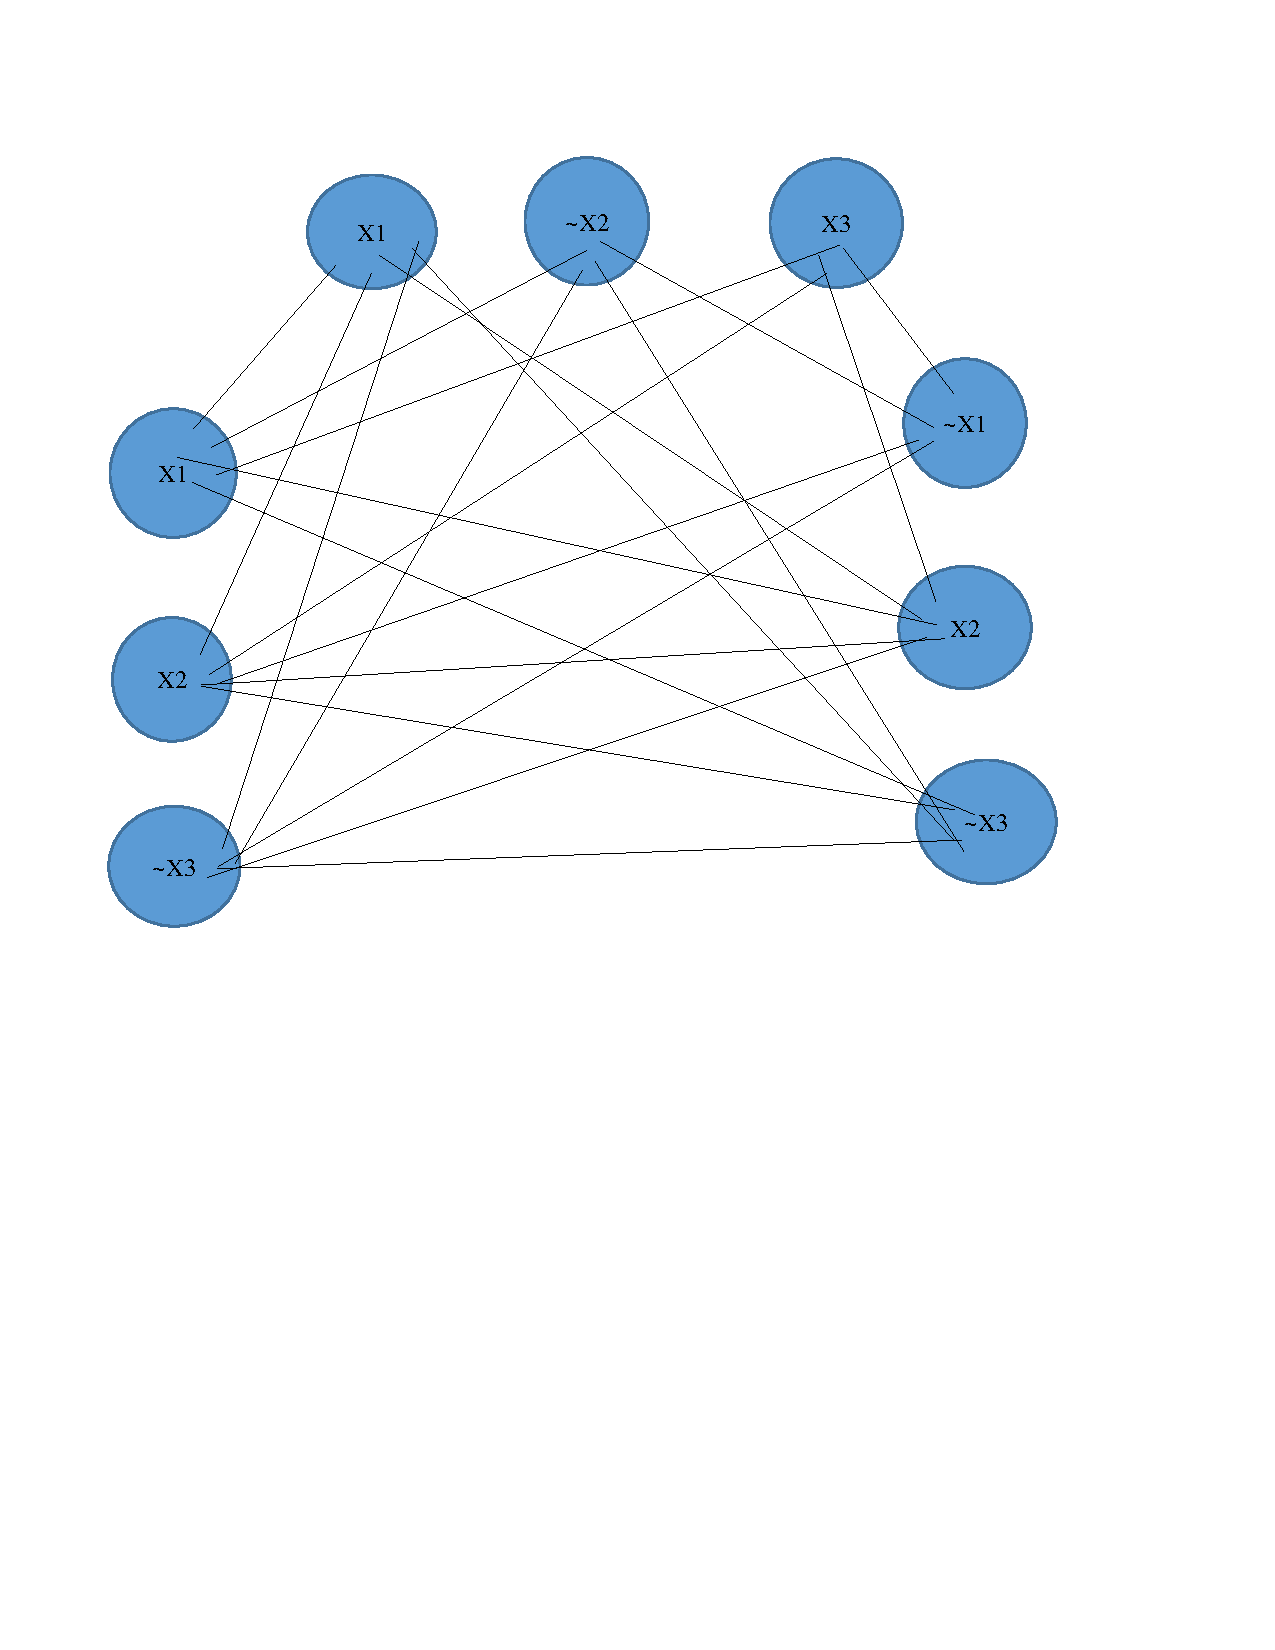
\includegraphics[scale=.80]{clique.pdf}
\end{figure}

There is a clique in this graph corresponding to X1 from the top triple, X2 from the left triple, and $\neg$ X3 from the right triple. Thus, the assignment X1 = 1, X2 = 1, and X3 = 0 is a satisfying assignment. (Note: This isn't the only satisfying assignment. X1 = 1, X2 = 1, X3 = 1 is also a satisfying assignment)

\end{document}